\snote{val}

Figure~3 of the main text compares the test $\chi^2/n$ of the reduced model with that of two references through their ratio. Supplementary Fig.~\ref{fig:valscatter} shows the same values as a scatter plot, which also displays their absolute level: points near $\chi^2/n=1$ predict at the level of the measurement noise, whereas points far above it (for example Okuonghae, Oliveira and Smith) are poorly fitted by every model, so that a favourable ratio there does not imply a good prediction. The values of every problem, the problems excluded from each panel and the reasons are listed in \texttt{paper/scirep/figure3/figure3\_heldout\_data.csv} of the repository, together with the script that produces both figures and checks every plotted point against that table.

\begin{figure}[!htb]
\centering
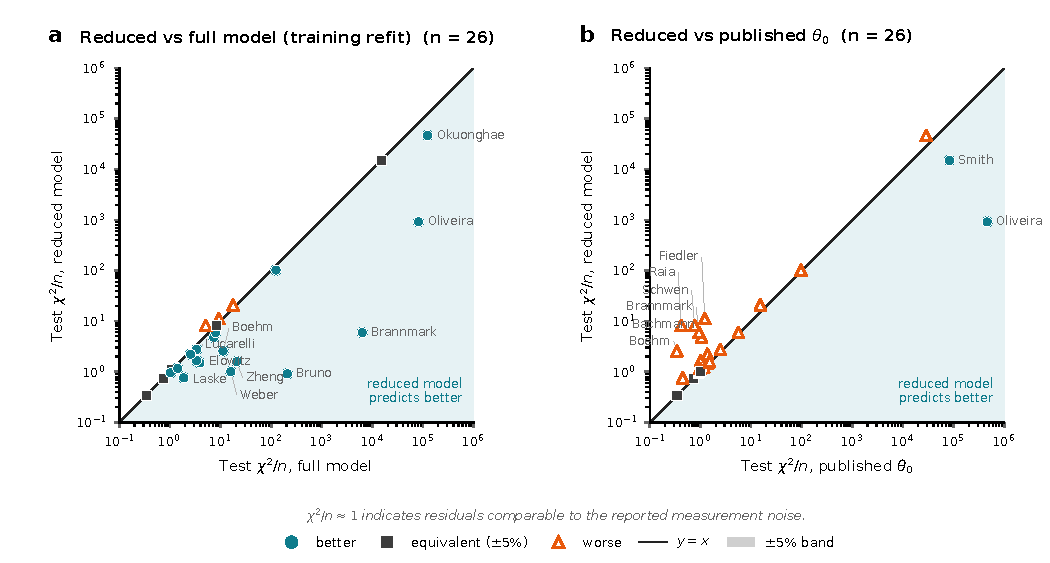
\includegraphics[width=\textwidth]{figures/figS1_validation_scatter.pdf}
\caption{\textbf{Prediction of held-out experiments, absolute values.} Test $\chi^2/n$ of the reduced model against \textbf{a}, the full model re-estimated on the same training data ($n=25$) and \textbf{b}, the published estimate $\theta_0$ ($n=27$), on logarithmic axes with the same scale. Solid line, $y=x$; grey band, equivalence within $\pm$5\%; shaded region, the reduced model predicts better. Circles, better; squares, equivalent; open triangles, worse. Names are shown for points away from the diagonal. The excluded problems are those of Figure~3.}
\label{fig:valscatter}
\end{figure}
